\documentclass{supervision}
\usepackage{course}

\Supervision{4}

\begin{document}
  \begin{questions}
    \SetQuestionNumber{12}
    \question \textit{Digital channels, modulation and transmission}
      \begin{parts}
        \part Explain the distinctions between baud rate and bit rate and
          between baseband and broadband.

        \part Why is synchronisation not an issue for transmission of
          analogue signals?

        \part What problem in synchronous transmission is Manchester coding
          designed to solve? Suggest a simpler but possibly more expensive
          way of solving the same problem. Explain why a system which has a
          slow but accurate oscillator would be more suited to asynchronous
          transmission than to synchronous transmission using Manchester
          coding.

        \part List three properties of a sinusoidal waveform which admit
          modulation. Explain the relationship between modulation and shift
          keying.
      \end{parts}

    %%%%%%%%%%%%%%%%%%%%%%%%%%%%%
    \section*{Topic 04 - Network}
    %%%%%%%%%%%%%%%%%%%%%%%%%%%%%

    \SetQuestionNumber{14}
    \question \textit{Switching}
      \begin{parts}
        \part Why is switching a practical necessity in large networks? In
          what way is switching a form of multiplexing?

        \part The switching process consists roughly of a demultiplexing
          stage, a routing stage and a remultiplexing stage. For each of the
          following examples of switching, explain what is being
          demultiplexed, what routing decisions are made, and how
          remultiplexing is performed:
          \begin{subparts}
            \subpart packet switching in the postal network;

            \subpart packet switching in an Ethernet switch;

            \subpart packet switching in an IP router;

            \subpart circuit switching in the telephone network;

            \subpart wave-division switching in an optical switch.

          \end{subparts}
        \part Switching can improve the efficiency of a network’s link
          utilisation, but may also cause problems. In a packet-switched
          network, two particular problems are increased latency and data
          loss.
          \begin{subparts}
            \subpart For one of the packet-switched examples above, explain
              how latency and loss might occur.

            \subpart Using the same example, suggest one way in which latency
              might be improved, and one way in which loss might be reduced.
              % more parallelism in the switch fabric
              % bigger buffers
              % or faster output lines for both

            \subpart To what extent are the problems of latency and loss less
              significant in circuit-switched networks? Give two
              disadvantages of circuit-switched networks over packet-switched
              networks.
              % latency: bounded (and small) by num hops, e.g. waiting 32 TSLs
              % per switch
              % loss: generally none, since uses reservations
              % coping with failure more difficult (hard state)
              % might not want constant capacity -> less efficient use of links

          \end{subparts}
      \end{parts}

    \SetQuestionNumber{16}
    \question \textit{General routing concerns}
      \begin{parts}
        \part Following are some examples of routing strategies and real
          systems which use them. For each one, suggest one reason why the
          strategy is a good choice, and another in which it might cause
          problems.

          \begin{subparts}
            \subpart flood routing in an Ethernet hub
              % good because no state involved; adapts to changes instantly
              % bad because burns capacity

            \subpart random routing in a peer-to-peer file-sharing network
              % no knowledge of topology needed
              % unbounded hop count -> many requests fail to reach destination

            \subpart source routing in the road network
              % if know topology, can play shortest/quickest route, loop-free
              % source does computation (no computation required within network)
              % but source needs to know topology (out of date atlas), and no
              % adaptability (road works)

            \subpart hot potato routing in crowded supermarket aisles (when
              heading for a target grocery shelf)

          \end{subparts}
        \part As well as benefits of bounded latency and assured capacity,
          circuit switching allows routing to be performed only once per
          connection, at set-up time. This contrasts with datagram-based
          routing, as commonly used in packet-switched networks, where
          routing is done for each datagram individually.

          \begin{subparts}
            \subpart Outline a set of additions or modifications to TCP/IP
              which would allow routing decisions to be made only once per
              TCP connection. Identify what (if any) other benefits of
              circuit switching your modifications provide, and which ones
              they do not.
              % modify routers to maintain per-flow state
              % need some end-to-end signalling (reservation) protocol like
              % RSVP, as part of connection set-up
              % other benefits are guaranteed capacity, bounded latency (and
              % jitter)
              % if have some kind of flowspec, can reserve buffer space and
              % link capacity admission control is based on buffer size and
              % output link rates
              % latency guarantee requires fair scheduling discipline with
              % deadline guarantees (“real-time”)

            \subpart Do your modifications preserve the reliability
              properties of datagram-based routing? Specifically, the
              property in question is that end-to-end connections can be
              maintained across a catastrophic failure of a router or link,
              assuming that an alternative path through the network exists.
              If they do, explain why. If not, suggest how this could be
              achieved, or explain why your modifications expressly preclude
              it.
              % “soft state”, i.e. times out, periodically regenerated
              % if re-routed, will eventually refresh state along different path
              % might have explicit re-routing notification, in order
              % to refresh state sooner, i.e. when router doesn’t recognise flow
              % it notifies sender, who refreshes state again (i.e. makes new
              % reservation)
              % if new route doesn’t have capacity, best-effort until next
              % state refresh cycle (repeats)
              % or maybe if can’t reserve capacity, last router in original
              % chain will keep trying new reroutes


          \end{subparts}
        \part You are required to design a topology discovery protocol for a
          network of switching nodes interconnected by links. There are $n$
          nodes, $l$ links, the maximum degree of any node is $k$ and there
          is a path between any two nodes of not more than $d$ hops. All
          links are bi-directional.

          Each node has a unique identifier of four bytes which it knows.

          \begin{subparts}
            \subpart Outline a protocol (including message formats) for a
              node to learn about its immediate neighbours.
              % There are numerous solutions in this space, here is one. Each
              % node sends out a message of the form
              %           |  TOPOLOGY PROBE |  NODE ID  |
              % each node receiving such a message replies with
              %           |  TOPOLOGY REPLY |  NODE ID  |
              % using its own NODE ID


            \subpart Design a protocol (including message formats) for
              distributing this information across the network.
              % There are numerous solutions in this space, here is one.
              % In order to build up the topology, it is not enough to simply
              % exchange information with immediate neighbours (aka next-hop
              % table).
              % each node in the network must receive neighbour information for
              % every other node.
              % For example a k (maximum degree) entry message of the form
              %      NEIGHBOURS  NODE ID
              %      Neighbour 1
              %      Neighbour 2
              %      ...
              %      Neighbour k (max)
              % would be flooded with a time to live count of d (diameter)

            \subpart Give a bound on the total amount of information which is
              transmitted to ensure that every node acquires complete
              topology information.

          \end{subparts}

        \part Consider a Distance-Vector Routing protocol. The routing
          table for node $A$ is expresed in a format where the rows
          indicate the destination and the columns indicate the first
          hop. That is, the number in (row $C$ column $D$) denotes the
          cost of the best currently known path to $C$ that starts with
          $A$ and sending to $D$. The initial table for Node $A$, before
          $A$ has exchanged any routing information with any other node,
          takes the form:

          \begin{table}[h]
            \centering
            \begin{tabular}{|c|ccc|}
              \hline
              Table for A & B        & C        & D        \\ \hline
              B           & 3        & $\infty$ & $\infty$ \\
              C           & 4        & 1        & $\infty$ \\
              D           & $\infty$ & $\infty$ & 2        \\
              E           & $\infty$ & $\infty$ & $\infty$ \\
              F           &          & $\infty$ & $\infty$ \\ \hline
            \end{tabular}
          \end{table}

          Note that in this initial routing table, A does not know paths
          to any destinations except its immediate neighbours.

          \begin{subparts}
            \subpart After $A$ receives a route update from $B$ ($B$ sends
              its initial table), what are the entries in the routing table
              for $A$?
              % answer in question sheet

            \subpart After $A$ receives a route update from $C$ ($C$ sends
              its initial table), what are the entries in the routing table
              for $A$?

            \subpart Assume now that all nodes exchange tables in an
              iterative process until steady-state is achieved. What are the
              steady-state entries in the table for node $A$?
          \end{subparts}

          \begin{figure}[h]
            \caption{A network topology. Numbers refer to the link-cost of
              indicated link.}
            \label{fig:1}
            \centering
              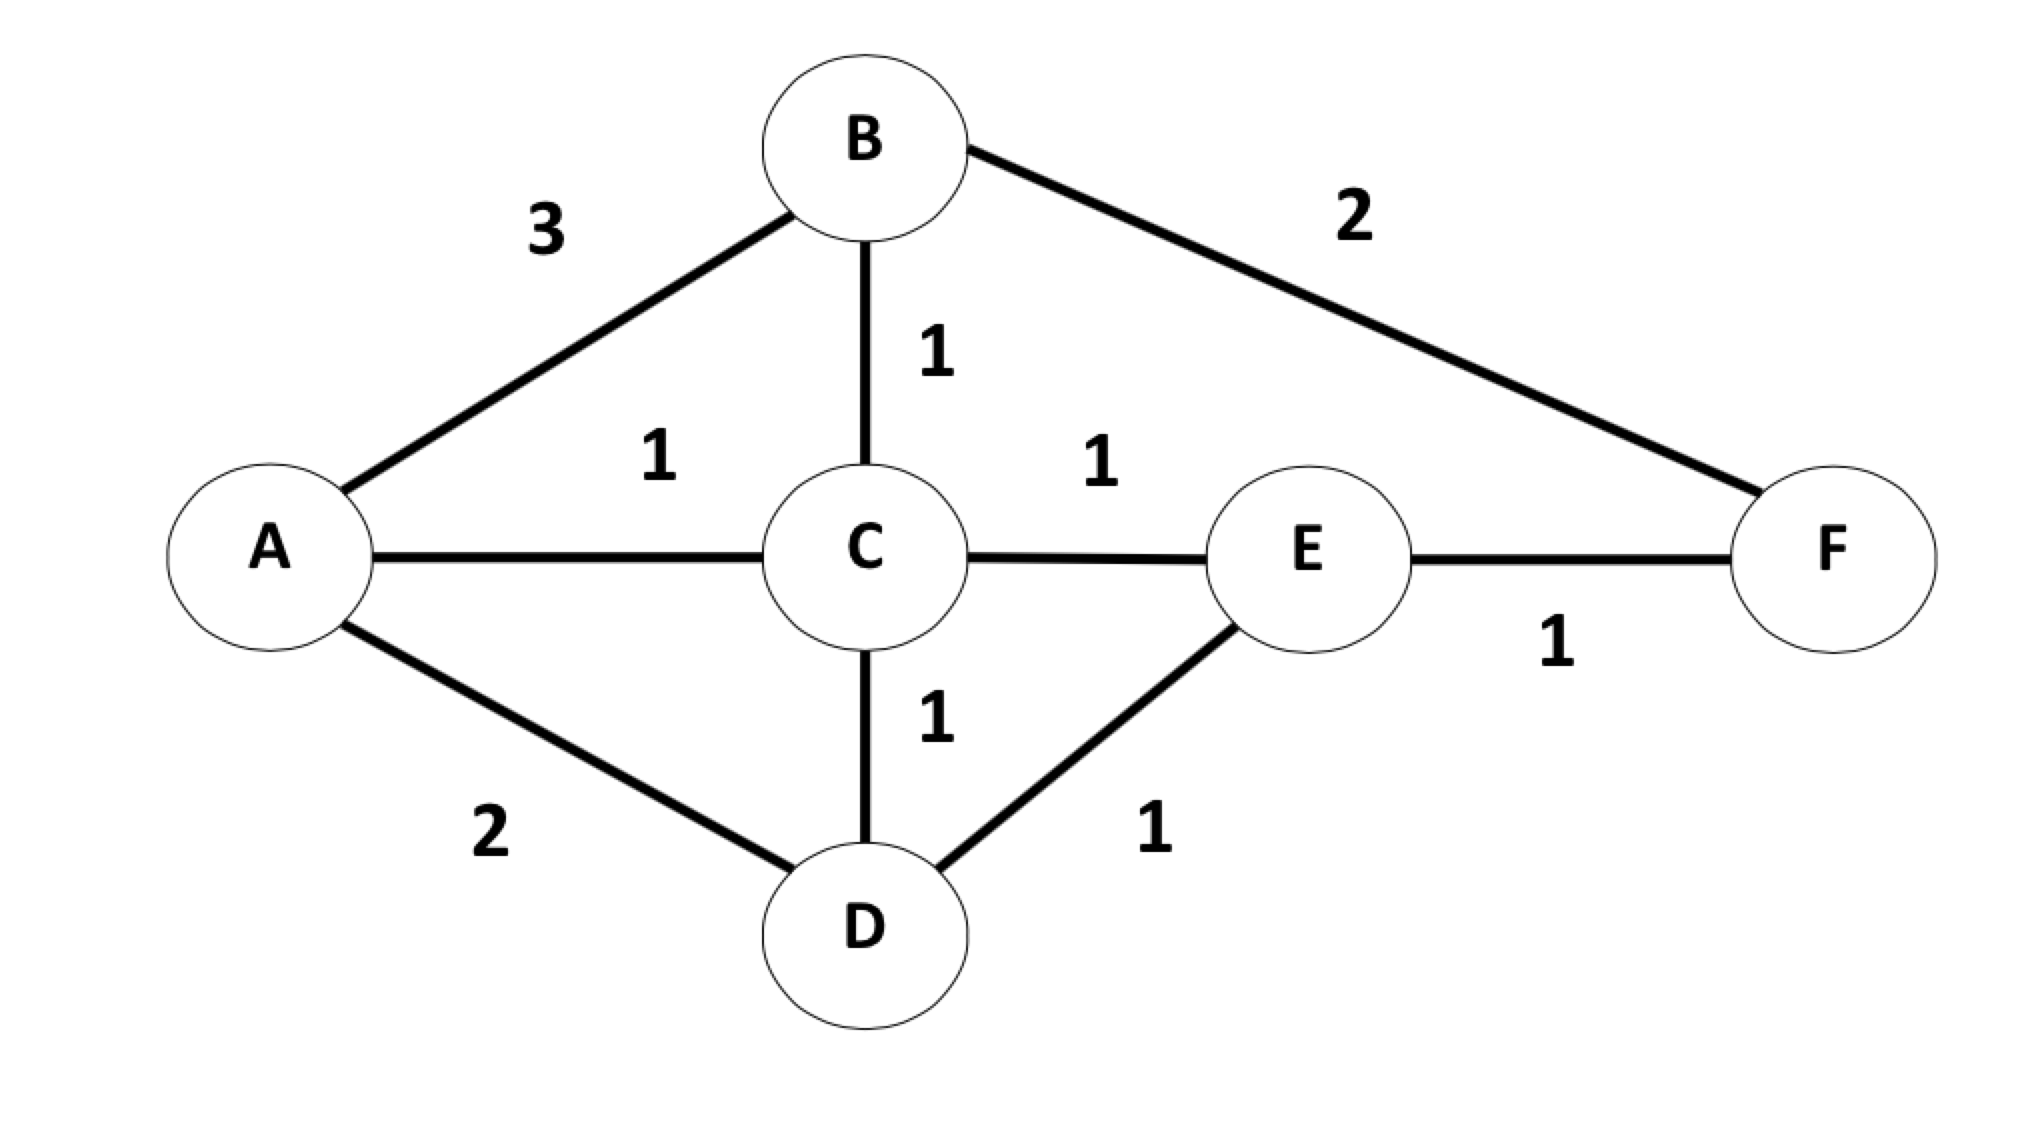
\includegraphics[width=0.75\textwidth]{16-figure-1}
          \end{figure}

          Now consider the network of Figure \ref{fig:1} and a Link-State
          Routing algorithm.

          \begin{subparts}
            \SetQuestionNumber{4}
            \subpart If $A$ sends a packet to $B$, what path does the packet
              take?

            \subpart If $A$ sends a packet to $F$, what path does the packet
              take?

            \subpart Now assume that the link cost for the links $C-E$ and
              $E-F$ both change to $6$. $E$ announces these changes and all
              nodes but $C$ get the update (that is, $C$ still thinks $C-E$
              and $E-F$ are link-cost $1$). Now $A$ sends to $F$, what path
              does the packet take?

            \subpart Finally, $C$ gets the new link-weight information and
              now knows that $C-E$ and $E-F$ are link-cost $6$. When $A$
              sends to $F$, what path does it take?

          \end{subparts}
      \end{parts}
    \question \textit{Supervision discussion questions}
      \begin{parts}
        \part Compare Forwarding versus Routing

        \part Compare and contrast Link-State Routing with Distance-Vector
          Routing. What are the (information) consistency models of each?
          What information is exchanged?

        \part What makes a fast LPM algorithm? (Longest-Prefix-Match)?

        \part What happens when (packet) fragment loss occurs?

        \part What is the state held by a NAT box? How does a NAT box work
          out its state?

        \part Why do packets tend towards the same path(route) through the
          network?

        \part How does ARP work?

        \part Compare DNS and ARP

        \part Why would I (or wouldn’t I) want to broadcast an ARP response?

        \part How does Gateway ARP do its thing?
      \end{parts}
  \end{questions}
\end{document}
